\chapter{Obbiettivi}\label{chapter:obbiettivi}
%%% Descrivo la situazione di partenza ovvero
%%% spiego ciò che abbiamo a disposizione con immagini ovvero configurazione chiusa e aperta
%%% inserisco che come primo obbiettivo ci siamo posti quello di creare uno shortest path non guidato
%%% poi abbiamo deciso di includere la funzione d'energia per guidare la ricerca
%%% le motivazioni che ci hanno spinto a fare questo lavoro --> Capisci come esprimerle
Sono stati creati molti framework che si occupano di trattare il problema del ripiegamento delle proteine, nessuno dei presenti metodi presta attenzione alle catene laterali dei singoli aminoacidi. 
Come descritto nel paragrafo \ref{subsec:Catena_laterale} tutti gli amminoacidi o quasi tutti hanno una catena laterale, che deve essere presa in considerazione quando si vanno ad effettuare delle rotazioni sulla struttura principale dell'amminoacido stesso. Chiaramente il problema non si verifica quando viene effettuata una rotazione su un singolo amminoacido, ma quando si lavora su proteine è necessario prestare attenzione affinché non vengano creati clash tra atomi appartenenti ad amminoacidi differenti. 


Come ampiamente descritto nella sezione precedente la glicoproteina spike gioca un ruolo fondamentale nella propagazione del virus SARS-CoV-2. Questa proteina è al centro di tutti gli studi indirizzati a cercare di neutralizzare per quanto possibile il virus o per lo meno cercare di minimizzare gli effetti sugli ospiti.
Il dipartimento di chimica mi ha fornito la proteina spike in due configurazioni quella chiusa e quella aperta, esse differiscono per lo stato in cui si trovano ovvero. La proteina spike nella versione chiusa, si trova in uno stato di pre fusione, mentre la proteina spike nello stato aperto è pronta a legarsi ad un recettore.
\begin{figure}
	\centering
	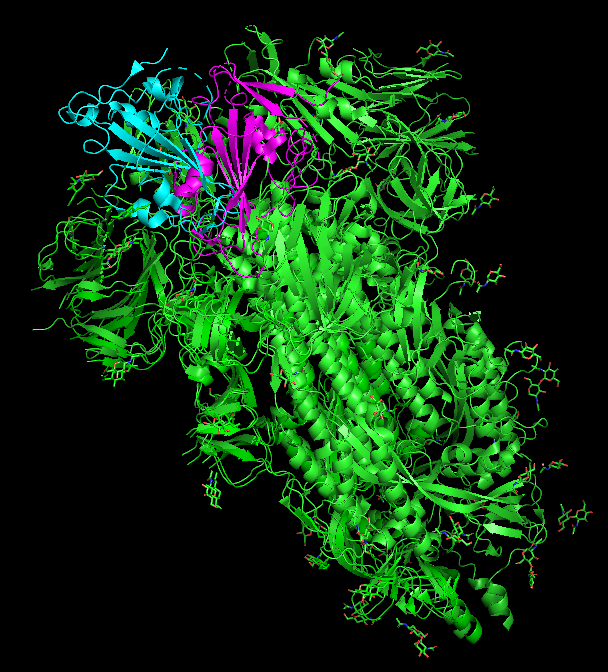
\includegraphics[width=0.6\textwidth]{Immagini/Struttura_aperta_chiusa.png}
	\caption{Abbiamo due configurazioni come detto in precedenza, la prima è quella chiusa contraddistinta dal colore magenta, mentre la seconda è quella aperta contraddistinta dal colore ciano.}
	\label{fig:Configurazioni}
\end{figure}
Una volta che abbiamo individuato le due configurazioni Fig.\ref{fig:Configurazioni} possiamo descrivere gli obbiettivi:
\vspace{10pt}
\begin{itemize}
	\item trovare lo shortest path tra le due configurazioni supponendo che il costo del singolo movimento sia 1;
	\vspace{5pt}
	\item trovare lo shortest path tra le due configurazioni utilizzando la funzione d'energia HINT per guidare la ricerca e pesare in modo il costo del singolo arco.
\end{itemize}

